\documentclass[10pt,twocolumn,letterpaper]{article}

\usepackage{cvpr}
\usepackage{times}
\usepackage{epsfig}
\usepackage{graphicx}
\usepackage{amsmath}
\usepackage{amssymb}

% Include other packages here, before hyperref.

% If you comment hyperref and then uncomment it, you should delete
% egpaper.aux before re-running latex.  (Or just hit 'q' on the first latex
% run, let it finish, and you should be clear).
\usepackage[breaklinks=true,bookmarks=false]{hyperref}

\cvprfinalcopy % *** Uncomment this line for the final submission

\def\cvprPaperID{****} % *** Enter the CVPR Paper ID here
\def\httilde{\mbox{\tt\raisebox{-.5ex}{\symbol{126}}}}

% Pages are numbered in submission mode, and unnumbered in camera-ready
%\ifcvprfinal\pagestyle{empty}\fi
\setcounter{page}{1}
\begin{document}

%%%%%%%%% TITLE
\title{Deep Learning Adversarial Network}

\author{Isingizwe Didier Frank\\
Tsinghua University\\
{\tt\small ididierfrank@yahoo.fr}
% For a paper whose authors are all at the same institution,
% omit the following lines up until the closing ``}''.
% Additional authors and addresses can be added with ``\and'',
% just like the second author.
% To save space, use either the email address or home page, not both
\and
Sui Ruoli\\
Tsinghua University\\
%{\tt\small srl19@mails.tsinghua.edu.cn}
\and
Bastien Bedu\\
Tsinghua University\\
%{\tt\small author@i2.org}
}

\maketitle
%\thispagestyle{empty}

%%%%%%%%% ABSTRACT
\begin{abstract}
   Generative adversarial networks (GANs) are algorithmic architectures
   that use two neural networks, pitting one against the other
   (thus the “adversarial”) in order to generate new, synthetic instances
   that can pass for real data. They are used widely in image generation,
   video generation and voice generation.  In this report we test the
   effectiveness of a GAN with self-attention (SAGAN) to generate real
   images of dog breeds. The task is following a kaggle competition. We
   find several challenges in training this model and evaluate the
   generations in the competition and in larger context of the field.
\end{abstract}

%%%%%%%%% BODY TEXT
\section{Introduction}

Generative methods are more and more viable with advances in deep learning
algorithms and more powerful training on larger datasets.
We are interested in exploring this potential in a fun way and looking at
photos of adorable pups at the same time. Dogs represent a good test case
also in another way because there are many distinguishable breeds that
humans can classify. Dog images on the internet are very abundant, behind
people and maybe only cats. For these reasons, a study on generating new
dog images from a distribution of training image breeds was chosen. These
experiments will provide insight generative methods using the adversarial
networks described next.

%-------------------------------------------------------------------------
\section{Background}

\subsection{GAN}

The Generative Adversarial Network (GAN) trains a generator and discriminator
network in tandem. The GAN class of machine learning systems was invented by
Ian Goodfellow in 2014. These methods are valuable for different reasons. For example,
generative methods such as the GAN can be used for data augmentation, 
and can mitigate the negative effects of having a limited training set
as in detecting a rare disease diagnosis, or labeling sparse images, etc.
GANs are advancingly used in state of the art creative frontiers. Unlike in
ML applications like prediction, there is no ground truth label. They
instead learn to mimic the domain which could be diverse: photographs,
drawing styles, musical styles, and writing styles. \cite{Authors14}

\begin{figure}
  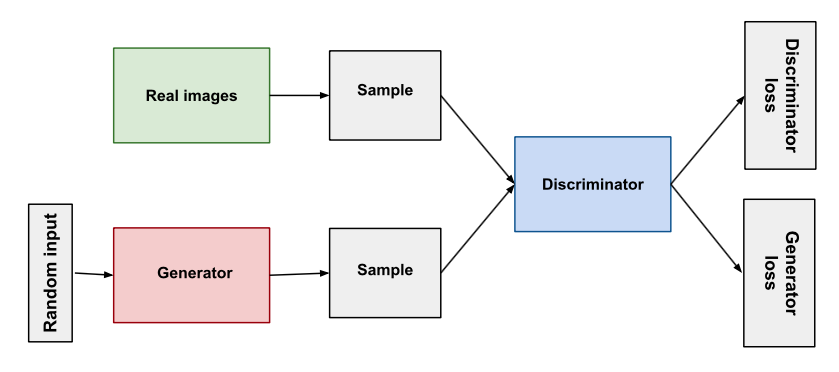
\includegraphics[width=1.0\linewidth]{images/gan.png}
  \caption{The GAN model.}
  \label{fig:gan}
\end{figure}

\begin{figure}
  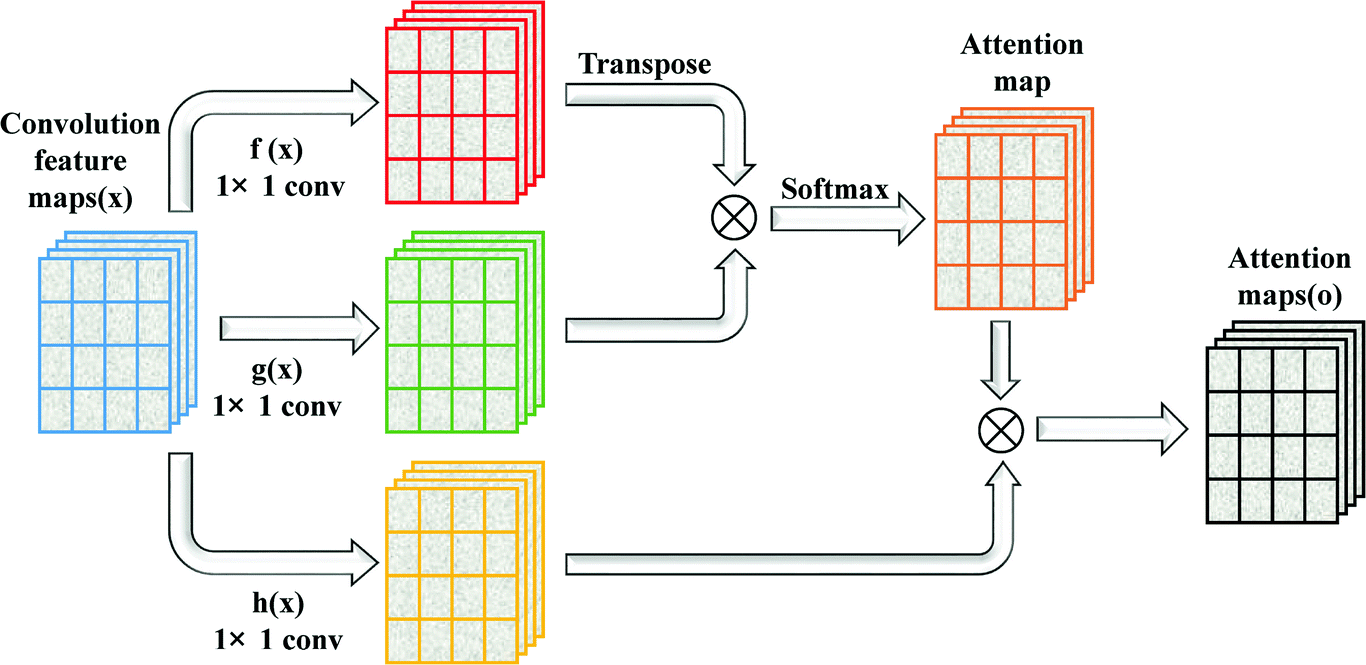
\includegraphics[width=1.0\linewidth]{images/sagan.png}
  \caption{The SAGAN model.}
  \label{fig:sagan}
\end{figure}

Through the adversarial process, the system learns
to generate new data that approximates the statistical distribution of the
training set. We can define the GAN as a minimax game between G and D where they
have a shared objective function V.

\begin{figure}
  
\includegraphics[width=1.1\linewidth]{images/gan_objective.png}
  \caption{The minimax objective game between D and G.}
  \label{fig:gan_objective}
\end{figure}

\subsection{SAGAN}

The Self-Attention Generative Adversarial Network (SAGAN) prioritizes the
appropriate long-range dependencies in an image. Higher resolution feature
maps are made more consistent with those in other parts of the image.
This is done through the self-attention mechanism. Attention mechanisms
have become very useful for models that need to capture correlations
between parts of an image (or other data) which would be difficult for
a convolutional kernel by comparison, because the receptive fields may not
cover the larger structures of interest and increasing filter size is computational
expensive. Furthermore the self-attention sometimes called intra-attention is a sequence method:
simply put, to calculate the response level it attends to all other positions
within the same sequence. These approaches saw much success in machine translation
and video sequence models. Explorations in the context of GANs have also been
promising. To refine the generator quality, SAGAN will consider the feature map
region within a contextual calculated area, the attention map, which asks as a mask
when rendering the location that attends it.

\begin{figure}
  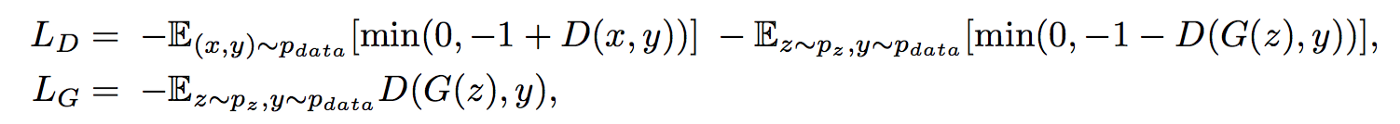
\includegraphics[width=1.1\linewidth]{images/sagan_hingeloss.png}
  \caption{The SAGAN hinge loss function.}
  \label{fig:sagan_hingeloss}
\end{figure}


%-------------------------------------------------------------------------
\section{Approach}

\subsection{The Kaggle Competition}

\small\begin{quote}
``This competition has an experimental format and submission style (images as submission).
Competitors must use generative methods to create their submission images and
are not permitted to make submissions that include any images already
classified as dogs or altered versions of such images."
\end{quote}

Evaluation in the competition was not done by qualitative manual inspection to provide an
objective basis for judging. Submissions in competition are evaluated on Memorization-
informed Fréchet Inception Distance (MiFID) where the smaller score means generated images
more closely match the real images. FID is a standard for evaluating GANs based on
extracting intermediate features from the Inception network. Two multivariate Gaussians
are fitted to the real and generated to calculate Fréchet distance.

\begin{align*}
  \text{FID} = ||\mu_r - \mu_g||^2 + \text{Tr} (\Sigma_r + \Sigma_g - 2 (\Sigma_r \Sigma_g)^{1/2})
\end{align*}

\begin{align*}
  d_{ij} = 1 - cos(f_{gi}, f_{rj}) = 1 - \frac{f_{gi} \cdot f_{rj}}{|f_{gi}| |f_{rj}|}
\end{align*}

\begin{align*}
  d = \frac{1}{N} \sum_{i} \min_j d_{ij}
\end{align*}

\begin{align*}
  MiFID = FID \cdot \frac{1}{d_{thr}}
\end{align*}

The thresholded distance is simply assigned 1 if d exceeds some pre-defined epsilon.

\subsection{Experiment}

The Stanford Dogs dataset contains images of 120 breeds of dogs from around the world.
The dataset was built with annotation from Imagenet and includes 20,580 examples
labeled by class. The dataset also includes bounding box annotations.

The training parameters were fixed at batch size of 32, 5 epochs of 5000 iterations
and using a hinge loss function. The SAGAN model architecture is as described above using
4 x 4 by 1024 channels fully connected node inputs. For regularization a batch
normalization layer is added before the rectified linear unit. We have followed the
advice to use a relatively lower generator learning rate (1e-4) and a relatively higher
discriminator learning rate (4e-4). Training the discriminator more is thought to reduce
output noise, thought noisiness was still problematic and significant difference was not
found for parity learning rate.

Fine details will require more computer resources to model. For this reason, many
low resolution or clipped images were submitted in the competition, see figure
\ref{fig:low_resolution}.

\begin{figure}
  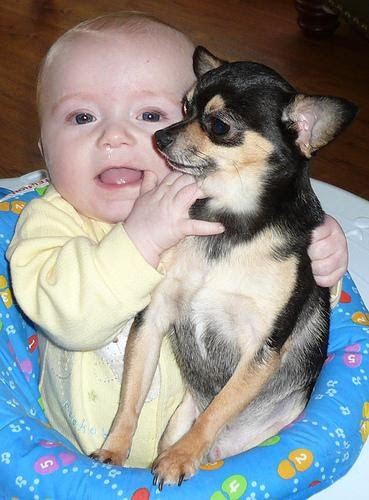
\includegraphics[width=0.7\linewidth]{images/confounder.jpg}
  \caption{An example image baby-with-dog which may confuse GAN training.}
  \label{fig:confouder}
\end{figure}

%-------------------------------------------------------------------------
\section{Conclusion}

GAN class methods like SAGAN are a powerful tool for generating new
data which is difficult to distinguish from its training examples.
But to open the full potential of these methods is difficult; there
are a wide range of results possible. As with other deep learning
method results are very dependent not only on network architecture but
also the dataset used and the computatation cycles available for
training your network. In general, generative models (which are
creating data) are considerable harder to train than the discriminative
models (that are processing data). In other words, it is easier to
recognize the "Mona Lisa" than to paint it.

\subsection{Expensive training and little data}

The Stanford Dogs Dataset also includes bounding box annotations. One improvment
that is possible would be to use the lower resolution images clipped around the
label of interest. This is because many training examples may be more confusing
for training than helpful, by including humans or multiple objects in the image,
and having many poses and views on the breeds to classify. These problems are
exacerbated by the per class rare data challenges. Paradoxically, with a
sufficiently strong generative model, the rare data problem would be solved.
Consider \ref{fig:imagenet_acc} which shows the Imagenet predicted accuracy
for each of the 120 classes at differences of 15 and 100 training examples.
The 15 example accuracy is generally roughly half. The maximum range is
nearly 57\%, for `African Hunting Dog', the only class besides `Dhole' to
exceed 50\%. On the other hand, there are several breeds which do not reach
10\% prediction accuracy even with 100 or more training examples. This
figure demonstrates the difficulty of prediction on this dataset, let alone
creating new and realistic images to match.

\begin{figure}
  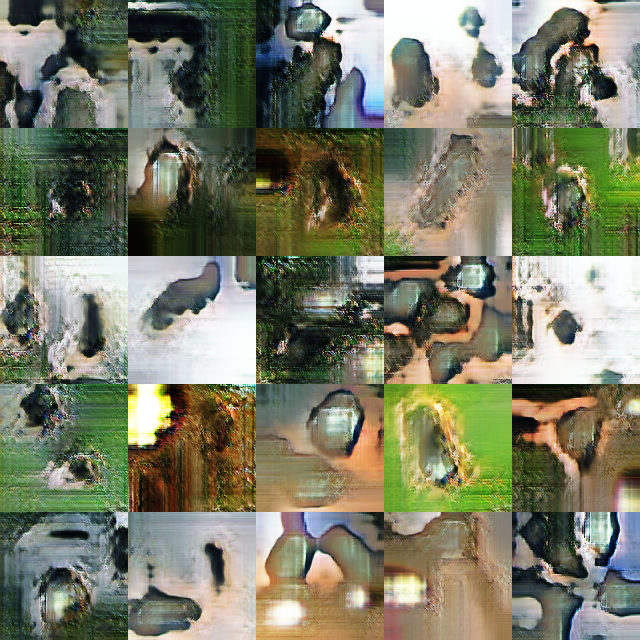
\includegraphics[width=0.8\linewidth]{images/results.png}
  \caption{Generative adversarial network dog image.}
  \label{fig:results}
\end{figure}


\begin{figure}
  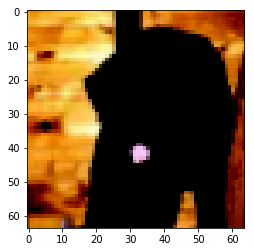
\includegraphics[width=0.8\linewidth]{images/low_resolution.png}
  \caption{A low resolution output from Kaggle.}
  \label{fig:low_resolution}
\end{figure}

%-------------------------------------------------------------------------
\section{Supplementary Material}

The experiment codes is available online
\href{https://github.com/FrankDidier/SAGAN-generation-of-pictures-of-dogs}{at Github}.
The training dataset is also available online
\href{http://vision.stanford.edu/aditya86/ImageNetDogs/}{Stanford Dogs Dataset}.
The Kaggle competition page is located
\href{https://www.kaggle.com/c/generative-dog-images/overview}{here}.

\begin{figure}
  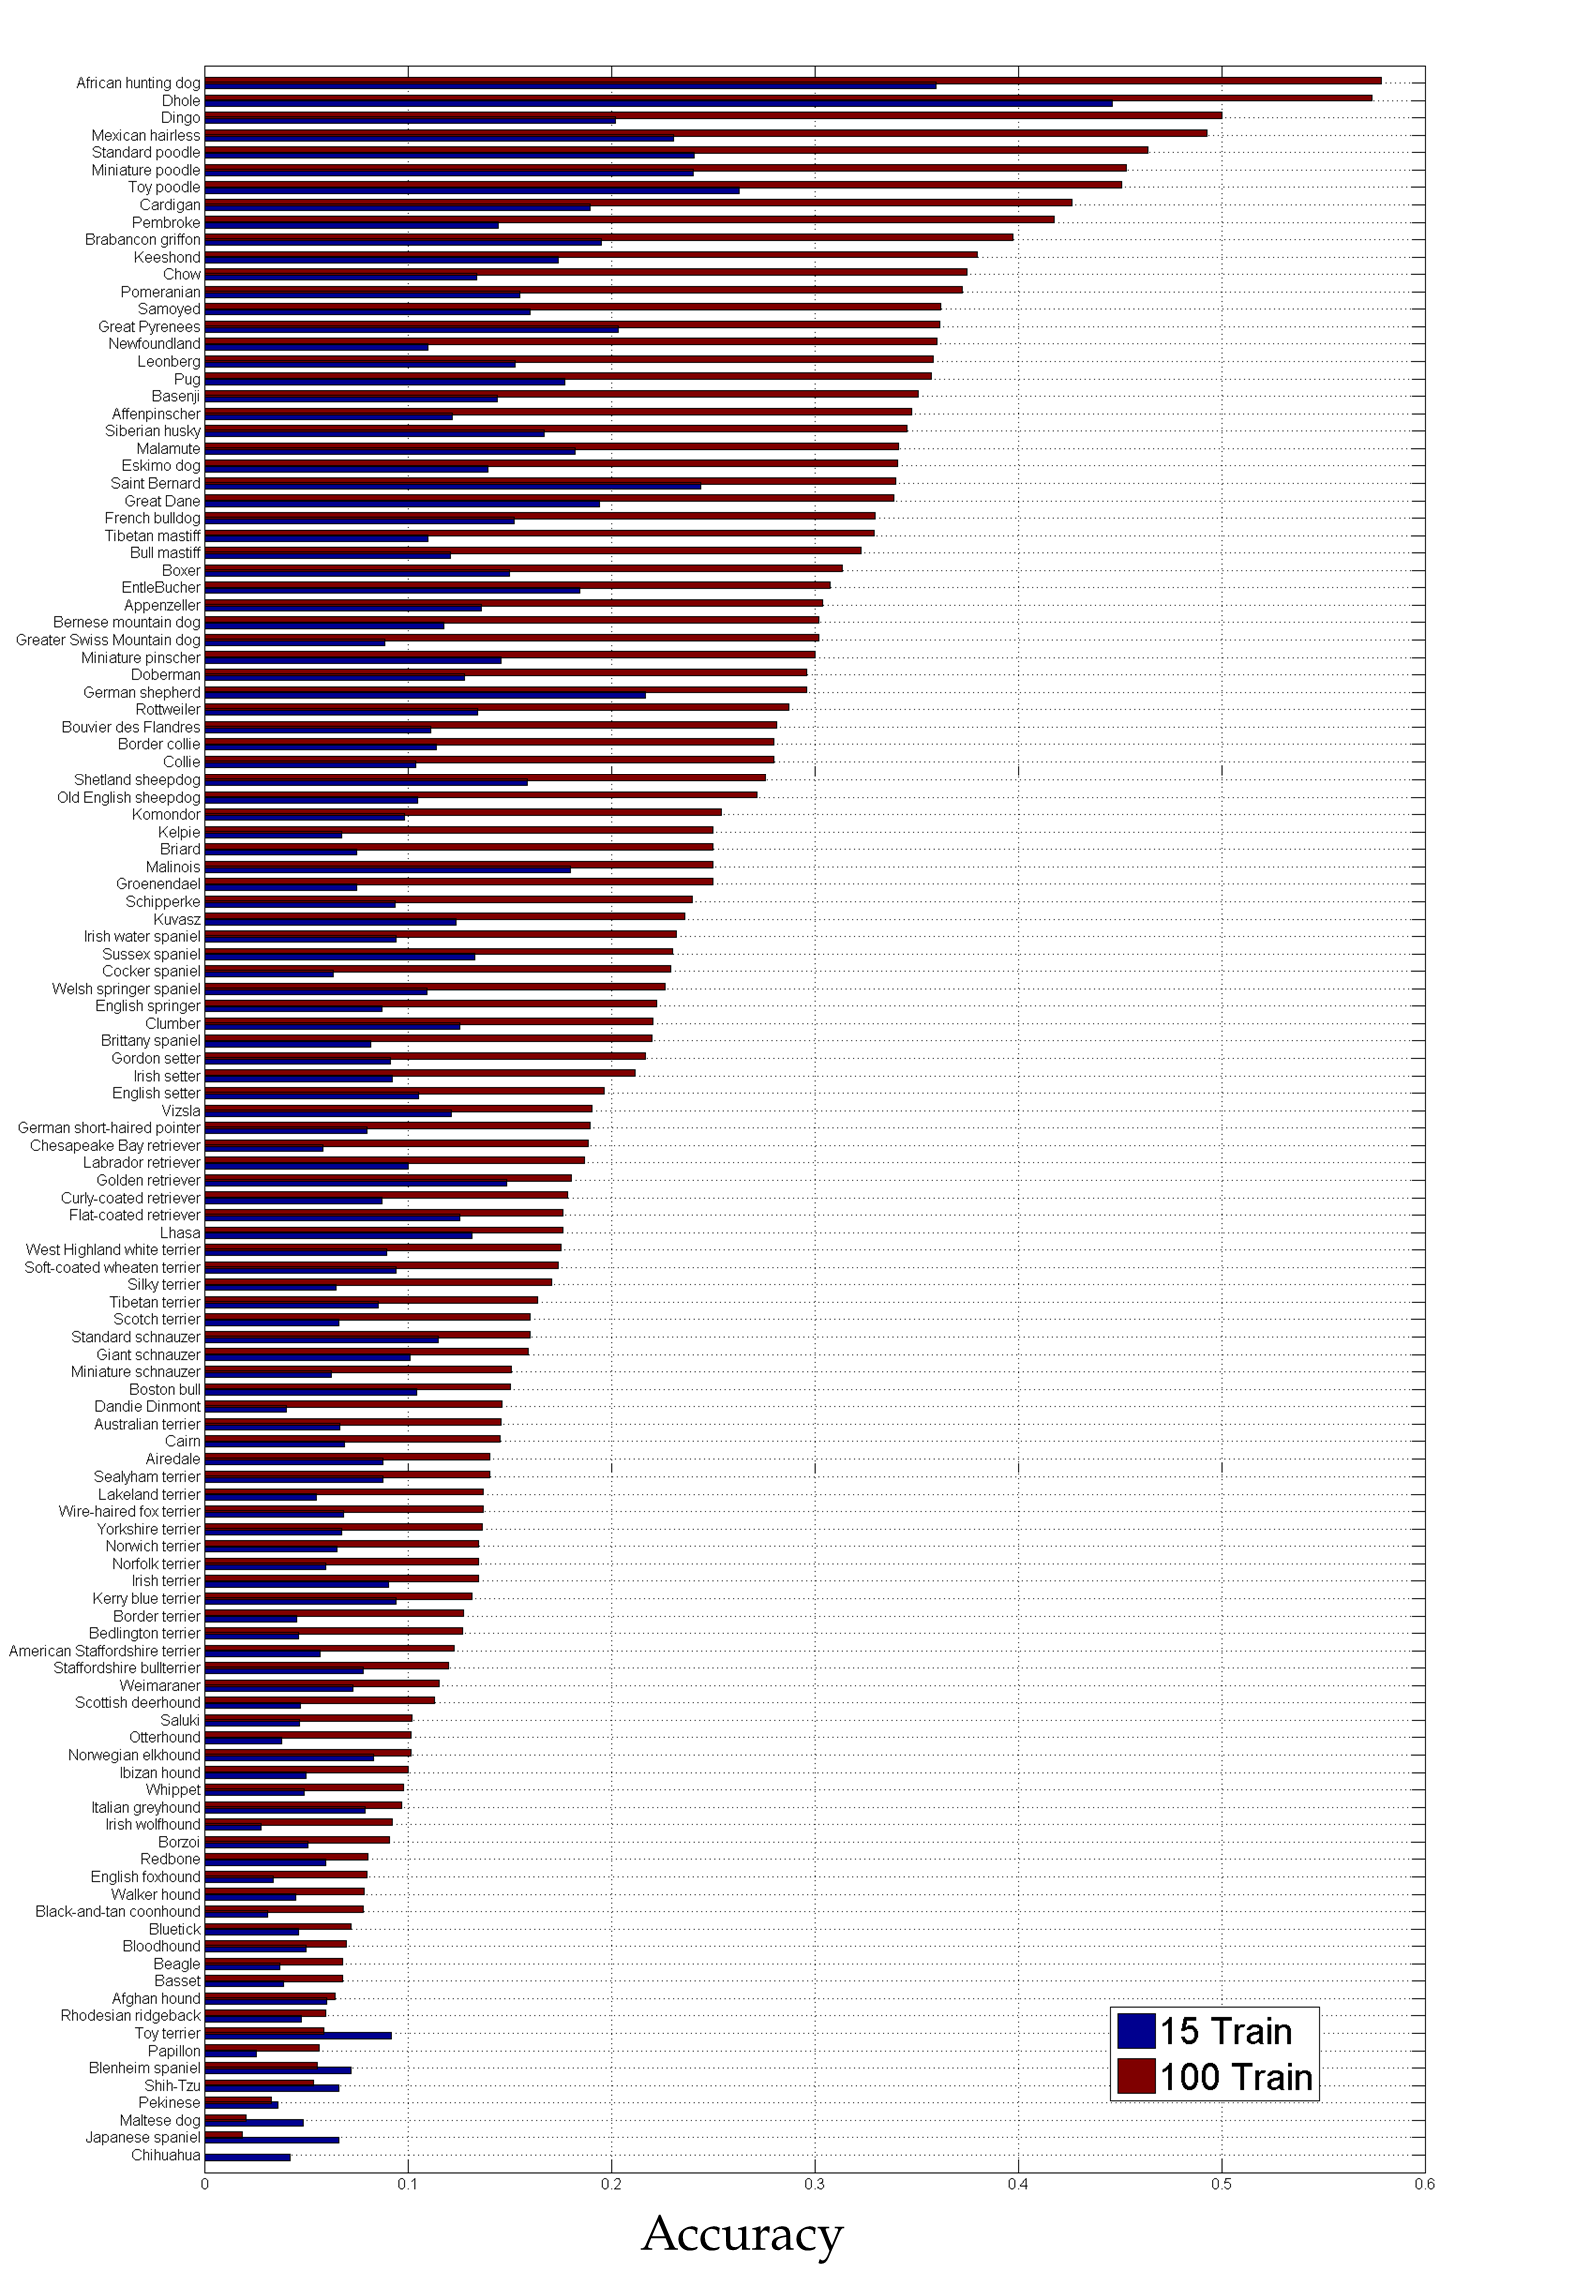
\includegraphics[width=1.0\linewidth]{images/imagenet_acc.png}
  \caption{Dogs breed accuracy of each for 15 and 100 training examples per class (Imagenet).}
  \label{fig:imagenet_acc}
\end{figure}

%-------------------------------------------------------------------------

\nocite{*}

{\small
\bibliographystyle{ieee}
\bibliography{fin}
}

%TODO fix bib

\end{document}
